\documentclass[fleqn]{article}
\usepackage{accsupp}
\usepackage{amssymb}
\usepackage{mathtools}
\usepackage{geometry}
\usepackage{graphics}
\usepackage[utf8]{inputenc} 
\usepackage[english]{babel}
\usepackage{tabularx}
\usepackage{lastpage}
\usepackage{listings}
\usepackage{xcolor}
\usepackage{courier}
\usepackage{url}
\geometry{
	a4paper,
	total={170mm,257mm},
	left=20mm,
	top=20mm,
}
\usepackage{fancyhdr}
\setlength{\headsep}{0pt}
\pagestyle{fancy} 
\rfoot{\thepage\ of \pageref{LastPage}}
\lfoot{Rover documentation: camera stream and browser control}
\cfoot{}
\renewcommand{\footrulewidth}{1pt}

\lstset{language=C, numbers=left, numberstyle=\small, basicstyle=\ttfamily\bfseries, showstringspaces=false, numbersep=10pt, numberblanklines=false, frame=single,  backgroundcolor=\color{mygray}, xleftmargin=15pt,  linewidth=1\linewidth,  breaklines=true, captionpos=b, tabsize=2, keywordstyle=\bfseries, morekeywords={package, class, final, new, WHILE, ENDWHILE, FOR, ENDFOR, IF, ENDIF, ELSE, SWITCH, CASE, ENDSWITCH}, escapeinside={*@}{@*}, breakindent=5pt}
%commentstyle=\color{olive},
\definecolor{mygray}{gray}{.95}

\begin{document}
\title{\rule{\textwidth}{1pt}\textbf{ Rover Documentation} \\ Tracing of Linux Processes and Threads using Rover Implementations \rule{\textwidth}{1pt}\vspace{-20pt}}
\date{}
\maketitle 
\setlength{\headsep}{20pt}
\vspace{-20pt}
\begin{tabularx}{\textwidth}{Xlll}
	& \textit{Version} & \textit{\today }&\\
	&\textit{Implementation} &\textit{Mustafa Özcelikörs} & \textit{mozcelikors@gmail.com}\\
	&\textit{Supervision \& revision} &\textit{Robert Höttger} &\textit{robert.hoettger@fh-dortmund.de}\\ \\
	&&\multicolumn{2}{l}{University of Applied Sciences and Arts Dortmund}\\ 
	&&\multicolumn{2}{l}{IDiAL Institute, Project AMALTHEA4public}\\
	&&\multicolumn{2}{l}{BMBF  	Fund.Nb. 01|S14029K} 
\end{tabularx} 
\vspace{15pt}\\
\begin{tabularx}{\textwidth}{cXc}
		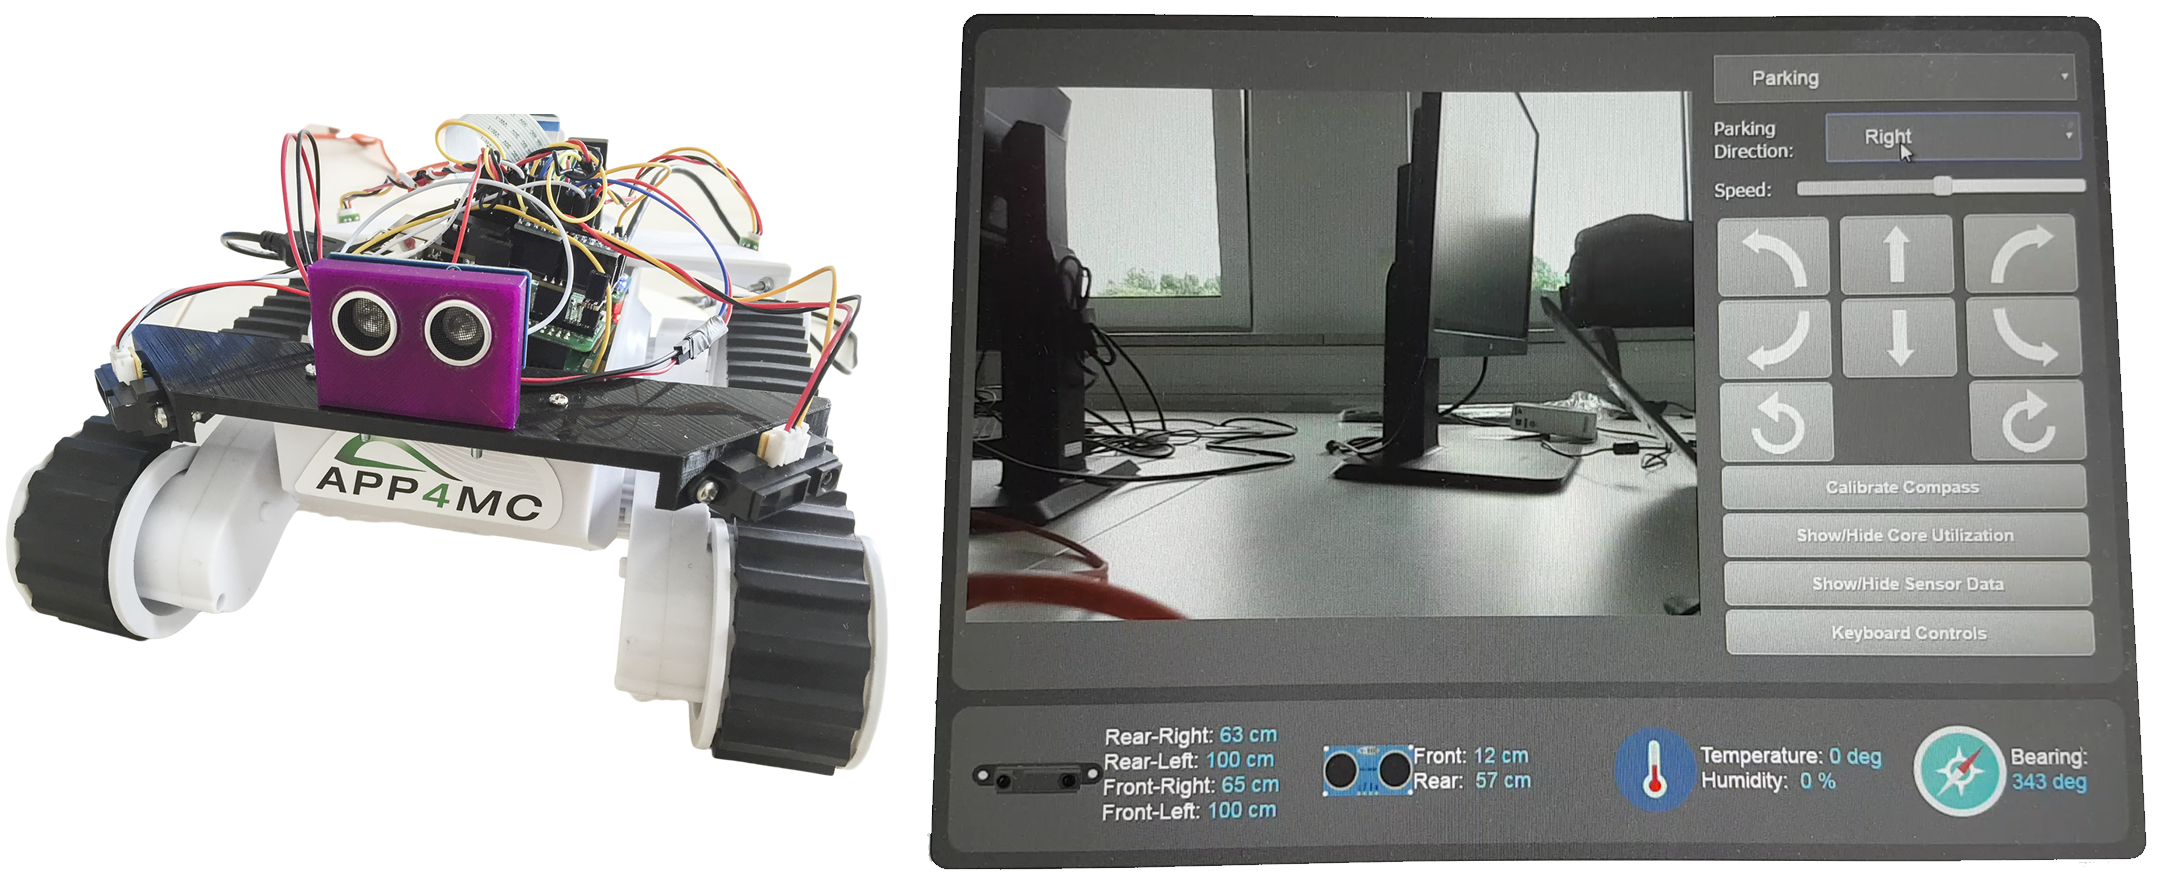
\includegraphics[width=0.5\textwidth]{rover.png}&&
		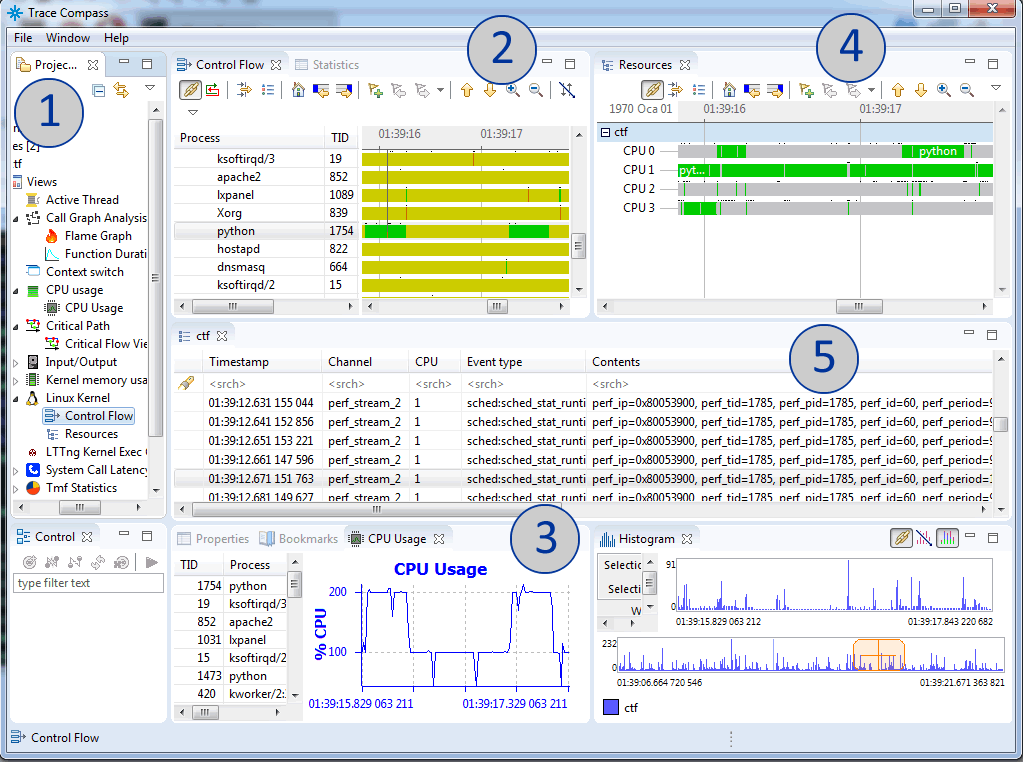
\includegraphics[width=0.42\textwidth]{tracecompass.png}
\end{tabularx}

\section{Scope}
This documentation explains how to use Perf module to generate traces in CTF (Common Tracing Format) format in order to take traces of Linux system processes and threads. How the trace conversion is performed and preliminary steps required to perform the trace conversion is also explained.
\section{Installing BabelTrace for Tracing}
The current distributions of perf does not allow data conversion functionality. Therefore, perf should be compiled from the Linux kernel with libbabeltrace support in order to be able to transform perf traces into CTF traces. To start with, one has to make sure that the repository list of the Raspberry Pi is up to date:
\begin{lstlisting}
	sudo apt-get update
\end{lstlisting}
In order to install the libbabeltrace from the repositories, following command can be used:
\begin{lstlisting}
	sudo apt-get install libbabeltrace-ctf-dev libbabeltrace-ctf1 libbabeltrace1 libbabeltrace-dev python3-babeltrace
\end{lstlisting}
To install the libbabeltrace from the source, which is required to compile perf with data conversion support, the following dependencies have to be installed:
\begin{lstlisting}
	sudo apt-get install dh-autoreconf bison libdw-dev libelf-dev flex uuid-dev libpopt-dev 
\end{lstlisting}
Next, following command can be used in order to clone, configure, build, and install the libbabeltrace from source:
\begin{lstlisting}
	sudo git clone git://git.efficios.com/babeltrace.git
	cd babeltrace
	sudo ./bootstrap
	sudo ./configure --prefix=/opt/libbabeltrace LDFLAGS=-L/usr/local/lib
	sudo make -j4 prefix=/opt/libbabeltrace
	sudo make install prefix=/opt/libbabeltrace
\end{lstlisting}
\section{Installing Perf with BabelTrace support from Source}
After the libbabeltrace is installed, perf should be rebuilt from Linux kernel with babeltrace support. Using the following command, the dependencies and features regarding the new perf build can be installed:
\begin{lstlisting}
	sudo apt-get install libnewt-dev binutils-arm-none-eabi libcrypto++-dev binutils-multiarch-dev libunwind-dev systemtap-sdt-dev libssl-dev libperl-dev libiberty-dev
\end{lstlisting}
Next, following command can be used in order to clone, build, and install a linux repository where the perf is available with data conversion support:
\begin{lstlisting}
	sudo git clone git://git.kernel.org/pub/scm/linux/kernel/git/acme/linux.git
	cd linux/tools/perf/
	sudo git checkout perf/core
	sudo LIBBABELTRACE=1 LIBBABELTRACE_DIR=/opt/libbabeltrace/ make
	sudo LIBBABELTRACE=1 LIBBABELTRACE_DIR=/opt/libbabeltrace/ make install
\end{lstlisting}
This will create a perf executable located at this directory: /linux/tools/perf/perf
\section{Tracing Processes and Threads}
\subsection{Option 1: Tracing Processes and Threads Manually}
In order to take a system trace for e.g. 15 seconds, the following command can be used while the applications are running:
\begin{lstlisting}
	sudo perf sched record -- sleep 15
\end{lstlisting}
This command will create a trace data in perf format, namely perf.data. Since Eclipse TraceCompass tool can not interpret perf format but it can interpret CTF format, the following command can be used to perform this transition:
\begin{lstlisting}
	sudo LD_LIBRARY_PATH=/opt/libbabeltrace/lib ./linux/tools/perf/perf data convert --to-ctf=./ctf
\end{lstlisting}
Keep in mind that the command above should be called at the path where perf.data is located. In order to avoid having to do this, the input argument can also be used to specify the location of the perf trace:
\begin{lstlisting}
	sudo LD_LIBRARY_PATH=/opt/libbabeltrace/lib ./linux/tools/perf/perf data convert -i=/path/to/perf.data --to-ctf=./ctf
\end{lstlisting}
In order to use the trace in an Eclipse TraceCompass on Windows operating system, the ctf trace could be archived by using the following command:
\begin{lstlisting}
	sudo tar -czvf trace.tar.gz ctf/
\end{lstlisting}

\subsection{Option 2: Tracing Processes and Threads Using Script}
In order to trace, and manually convert the trace, create a script with the following content:
\begin{lstlisting}
	#!/bin/bash
	args=("$@")
	trace_name=${args[0]}
	seconds=${args[1]}
	perf_directory=${args[2]}
	
	if [ "$#" -ne 3 ]; then
		echo "Entered arguments seem to be incorrect"
		echo "Right usage: sudo TraceLinuxProcesses.sh <trace_name> <period> <path_to_perf>"
		echo "e.g. sudo TraceLinuxProcesses.sh APP4MC_Trace 15 /home/pi/linux/tools/perf"
	else
		echo "### Creating directory.."
		sudo mkdir out_$trace_name/
		echo "### Writing out process names.."
		ps -aux >> out_$trace_name/Processes_List.txt
		echo "### Tracing with perf for $seconds seconds.."
		sudo $perf_directory/./perf sched record -o out_$trace_name/perf.data -- sleep $seconds
		echo "### Converting to data to CTF (Common Tracing Format).."
		sudo LD_LIBRARY_PATH=/opt/libbabeltrace/lib $perf_directory/./perf data convert -i out_$trace_name/perf.data --to-ctf=./ctf
		sudo tar -czvf out_$trace_name/trace.tar.gz ctf/
		sudo rm -rf ctf/
		
		echo "### Process IDs are written to out_$trace_name/Processes_List.txt"
		echo "### Trace in Perf format is written to out_$trace_name/perf.data"
		echo "### Trace in CTF format is written to out_$trace_name/trace.tar.gz"
		echo "### Exiting.."
	fi
\end{lstlisting}
Now, save this script with the name TraceLinuxProcess.sh, and grant privileges by using:
\begin{lstlisting}
	sudo chmod 777 TraceLinuxProcesses.sh
\end{lstlisting}
The provided script takes the three arguments: trace name, amount of time to trace, installed perf directory. An example way to call this script is shown below which traces the system for 15 seconds using the perf object located at /home/pi/linux/tools/perf/ directory:
\begin{lstlisting}
	sudo TraceLinuxProcesses.sh APP4MC_Trace 15 /home/pi/linux/tools/perf
\end{lstlisting}
The script produces an output directory which contains perf format data, ctf format and the process id list to interpret the output. 

\section{Visualization and Interpretation of the Trace}
By using Eclipse TraceCompass, which can be downloaded from \textit{http://www.eclipse.com/tracecompass}, traces in CTF format can be interpreted. By choosing the trace file by selecting \textit{File} and then \textit{Import} menu items, the trace can be imported into Eclipse TraceCompass. Eclipse TraceCompass is shown in the Figure \ref{fig:tracecompass}.

TraceCompass enables users to look at their system using several views such as call graphs, threads, context switches, cpu usage, critical path, I/O, control flow, and resources which can be seen as (1) in the figure. Control flow window (2) shows each process state with respect to time including the transitions along all the processes. System-wide CPU usage and individual processes' CPU usages are shown in the CPU Usage window which is shown as (3) in the figure. Therefore, if the system has 4 cores, the CPU usage of up to 400 percent could be observed. Resources window (shown as (4)) depicts how processes are distributed amongst the existing cores with respect to time. Therefore, the load balancing could be roughly observed from this view by simply looking at each of the cores. Moreover, using the Resources window, one can measure and estimate the timing properties of the schedule of the system. Finally, the trace event list (shown as (5)) can be used to see exact events that occurred in a specific time by selecting a time frame from other windows.

\begin{figure}[!ht]
	\centering
	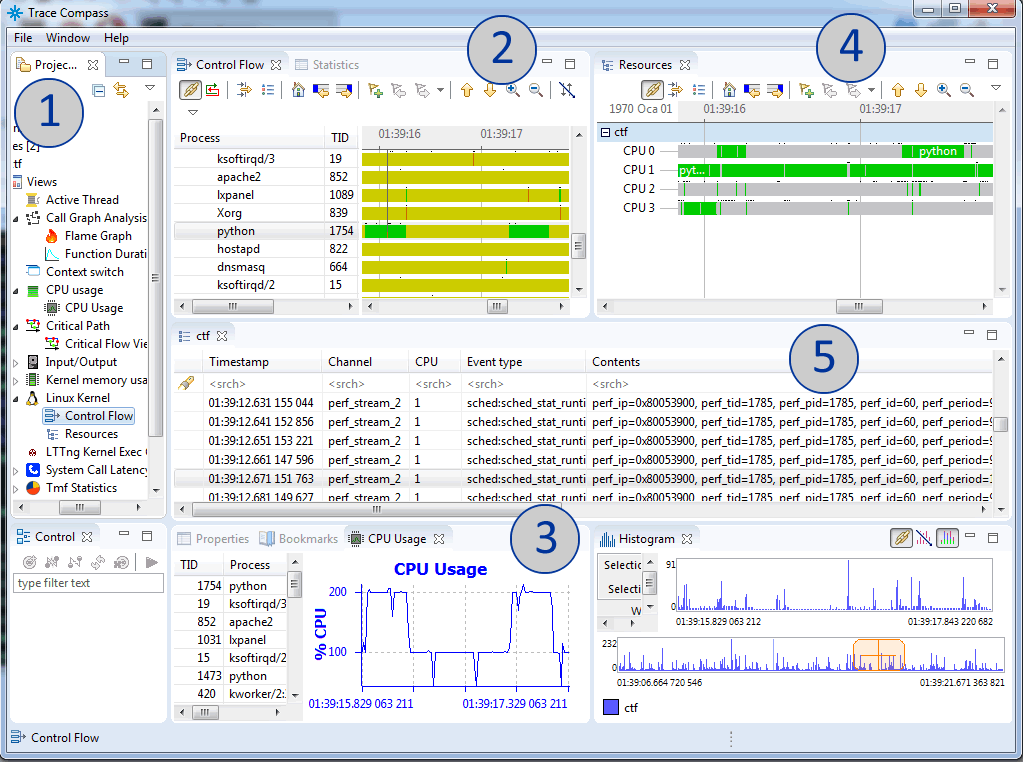
\includegraphics[scale=0.44]{tracecompass.png}
	\caption{Eclipse TraceCompass}
	\label{fig:tracecompass}
\end{figure}

\end{document}